\documentclass[tikz,border=2pt]{standalone}
\usepackage{amsmath,amssymb}
\usepackage{pgfplots}
\pgfplotsset{compat=1.18}
\usetikzlibrary{arrows.meta}

\begin{document}
% sin x with its Taylor polynomials around 0: P_1(x) = x (left) and P_3(x) = x - x^3/3! (right);
% the cubic stays close to sin x on a wider interval.
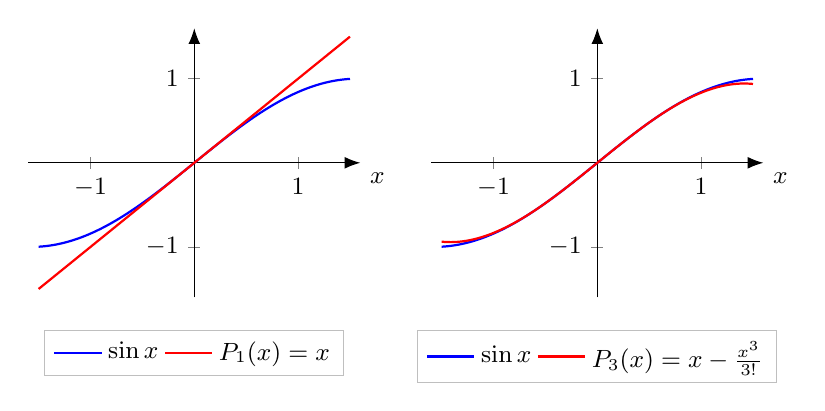
\begin{tikzpicture}[every node/.style={font=\small}]
	\pgfplotsset{tp/.style={
		width=5.8cm, height=5cm,
		axis lines=middle, axis line style={-{Latex[length=2mm]}},
		xmin=-1.6, xmax=1.6, ymin=-1.6, ymax=1.6,
		xtick={-1,1}, ytick={-1,1},
		tick label style={font=\small},
		xlabel={$x$}, xlabel style={below right},
		domain=-1.5:1.5, samples=100, clip=false,
		legend style={at={(0.5,-0.12)}, anchor=north}, legend columns=2, legend cell align={left},
		legend style={font=\small, draw=gray!50, fill=white}}}
	\begin{axis}[tp, name=left]
		\addplot[blue, thick] {sin(deg(x))};
		\addlegendentry{$\sin x$}
		\addplot[red, thick] {x};
		\addlegendentry{$P_1(x)=x$}
	\end{axis}
	\begin{axis}[tp, at={(left.east)}, anchor=west, xshift=0.9cm]
		\addplot[blue, thick] {sin(deg(x))};
		\addlegendentry{$\sin x$}
		\addplot[red, thick] {x-x^3/6};
		\addlegendentry{$P_3(x)=x-\frac{x^3}{3!}$}
	\end{axis}
\end{tikzpicture}
\end{document}
